\documentclass[11pt, spanish]{report}
\usepackage[spanish]{babel}
\usepackage[utf8]{inputenc}
\usepackage{geometry}
\usepackage{graphicx}
 \geometry{
 a4paper,
 total={170mm,257mm},
 left=20mm,
 top=20mm,
 }
\usepackage{graphicx}
\graphicspath{ {images/} }
\usepackage[utf8]{inputenc}
\decimalpoint

\title{Evaluación2}
\author{César Andrés Pérez Robinson }
\date{Mayo 2019}

\begin{document}

\maketitle

\section{Introducción}
A continuación se muestra el desarrollo y resultados de la actividad de Evaluación numero dos, la cual está divida en tres partes, y se analizan dos archivos de datos, meteorológicos y de flujos de un viñedo del 2018.
\subsection{PARTE UNO}
En esta parte se requiere recrear una tabla presentada por Djaman (2018), la cual muestra la variación mensual promedio de la velocidad del viento, temperatura promedio, máxima y mínima, humedad relativa promedio, máxima y mínima y la radiación neta \\
Utilizando jupyter notebook se realizan los pasos comunes, descargar las bibliotecas y subir los archivos de datos. Se observa que el archivo de datos meteorológicos presentan dos variables para la medición del tiempo, 'Date' y 'Time' las cuales son modificadas para poder crear una variable tipo datetime, usando:
\begin{verbatim}
# para hacer la variable de fecha
df1["FECHA"] = df1["Date"] +" "+ df1["Time"]
df1['FECHA'] = pd.to_datetime(df1.apply(lambda x: x['FECHA'], 1), dayfirst=True)
df1.drop( ["Date","Time"], axis=1, inplace=True )
\end{verbatim}
Después se filtra el DataFrame con tal de quedarse con las columnas de interés, y se agregan las variables 'MES' y 'DIA' a partir de la función dt.month y dt.day. \\
Para agregar al DataFrame aquellas columnas de interes, las cuales muestren los promedios obtenidos de las variables mencionadas anteriormente se crea otro DataFrame y se agregan ahí dichas variables utilizando:
\begin{verbatim}
# agregando al dataframe las columnas que nos interesan
dfm_mes = pd.DataFrame()
dfm_mes['V_Viento(m/s)'] = np.round(dfm.groupby(["MES"])["WS_ms_S_WVT"]
        .transform("mean"), decimals=2)
dfm_mes['Tmax'] = np.round(dfm.groupby(["MES"])["AirTC_Avg"]
        .transform("max"), decimals=2)
dfm_mes['Tmin'] = np.round(dfm.groupby(["MES"])["AirTC_Avg"]
        .transform("min"), decimals=2)
dfm_mes['Tprom'] = np.round(dfm.groupby(["MES"])["AirTC_Avg"]
        .transform("mean"), decimals=2)
dfm_mes['RHmax'] = np.round(dfm.groupby(["MES"])["RH"]
        .transform("max"), decimals=2)
dfm_mes['RHmin'] = np.round(dfm.groupby(["MES"])["RH"]
        .transform("min"), decimals=2)
dfm_mes['RHprom'] = np.round(dfm.groupby(["MES"])["RH"]
        .transform("mean"), decimals=2)
dfm_mes['Radiación'] = np.round(dfm.groupby(["MES"])["Rn_Avg"]
        .transform("mean"), decimals=2)
dfm_mes['Albedo'] = np.round(dfm.groupby(["MES"])["albedo_Avg"]
        .transform("mean"), decimals=2)

dfm_mes=dfm_mes.drop_duplicates(subset=['V_Viento(m/s)','Tmax',
    'Tmin','Tprom','RHmax','RHmin','RHprom','Radiación','Albedo'])
\end{verbatim}
Se eliminan los duplicados con tal de que solamente se muestre un renglón para cada mes. Se obtiene la Figura 1
\begin{figure}[ht]
\caption{Renglón para cada mes}
\centering
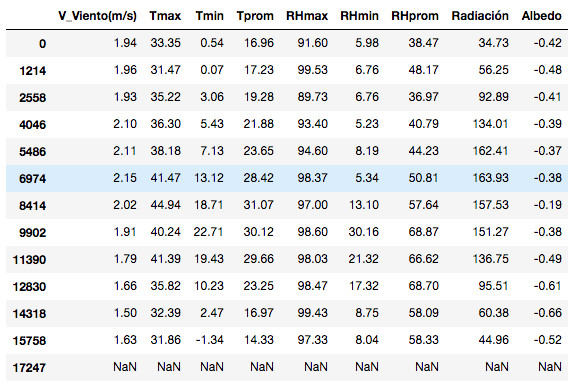
\includegraphics[width=0.65\textwidth]{dfm_mes.png}
\end{figure}
Se elimina el último renglón de la Figura 1 y se agrega una columna de los meses con:
\begin{verbatim}
mes=["Enero",'Febrero','Marzo','Abril','Mayo','Junio','Julio',
'Agosto','Septiembre','Octubre','Noviembre','Diciembre']
dfm_mes['MES']=mes
\end{verbatim}
Se grafican las temperaturas máximas, mínimas y promedio en la Figura 2, utilizando:
\begin{verbatim}
# Temperaturas máxima, mínima y promedio
X = mes                 
N = np.arange(12)         
Ymax = dfm_mes['Tmax']     
Ymin = dfm_mes['Tmin']     
Yprom = dfm_mes['Tprom']     


plt.plot(Ymax, label = 'Máxima', color = 'firebrick')   
plt.plot(Ymin, label = 'Mínima', color = 'steelblue')   
plt.plot(Yprom, label = 'Promedio', color = 'forestgreen')   

plt.xticks(N, X, size = 'medium', rotation = 45)  
plt.ylabel("Temperatura (ºC)")  
plt.legend()
plt.grid()
plt.title('Temperaturas mensuales en 2018')
plt.show()
\end{verbatim}
\begin{figure}[ht]
\caption{Temperaturas mensuales del 2018}
\centering
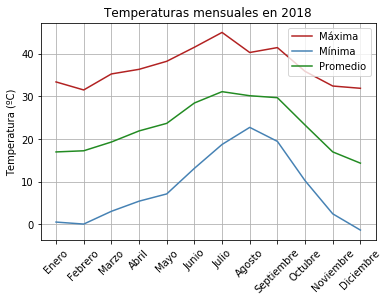
\includegraphics[width=0.65\textwidth]{figura2.png}
\end{figure}
La radiación solar promedio para cada mes del 2018 se muestra en la Figura 3 utilizando:
\begin{verbatim}
# Radiación solar
X = mes                 
N = np.arange(12)         
Rad = dfm_mes['Radiación']     

plt.plot(Rad, label = 'Radiación Solar', color = 'darkorange')   

plt.xticks(N, X, size = 'medium', rotation = 45)  
plt.ylabel("Radiación Solar")  
plt.legend()
plt.grid()
plt.title('Radiación Solar Mensual en 2018')
plt.show()
\end{verbatim}
\begin{figure}[ht]
\caption{Variación mensual de Radiación Solar}
\centering
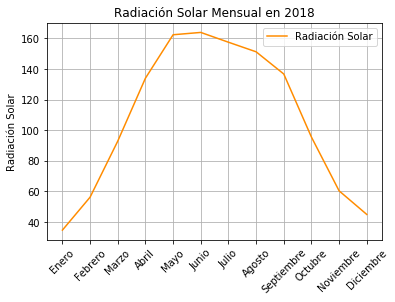
\includegraphics[width=0.65\textwidth]{figura3.png}
\end{figure}
Por último para la parte 1, se muestra en la Figura 4 la humedad relativa máxima, mínima y promedio utilizando:
\begin{verbatim}
# Humedar Relativa; máxima, mínima y promedio
X = mes                 
N = np.arange(12)         
Ymax = dfm_mes['RHmax']     
Ymin = dfm_mes['RHmin']     
Yprom = dfm_mes['RHprom']     


plt.plot(Ymax, label = 'Máxima', color = 'lightcoral')   
plt.plot(Ymin, label = 'Mínima', color = 'skyblue')   
plt.plot(Yprom, label = 'Promedio', color = 'seagreen')   

plt.xticks(N, X, size = 'medium', rotation = 45)  
plt.ylabel("Humedad Relativa")  
plt.legend()
plt.grid()
plt.title('Humedad Relativa Mensual en 2018')
plt.show()
\end{verbatim}
\begin{figure}[ht]
\caption{Variación mensual de Humedad Relativa}
\centering
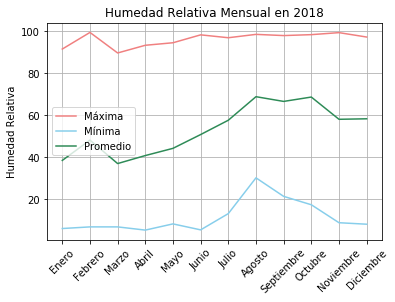
\includegraphics[width=0.65\textwidth]{figura4.png}
\end{figure}
\subsection{PARTE DOS}
En esta parte se estima la Evapotranspiración ET0 mensual promedio, utilizando tres ecuaciones de autores presentados en el artículo de Djaman (2018). \\
\begin{equation}
ET_0=(0.0252T+0.078)Rs
\end{equation}
La ecuación (1) es de Jensen y Haise (1963) y fue utilizada con:
\begin{verbatim}
# Ec 07 - Jansen & Haise (1963), ETo =(0.0252T + 0.078)Rs 
EvapT07 = []
for i in range (0,len(dfm_mes)):
    ET = (0.0252*dfm_mes['Tprom'][i]+0.078)*dfm_mes['Radiación'][i]
    EvapT07.append(ET)
\end{verbatim}
\begin{equation}
ET_0=0.0393Rs(Tmean+9.5)^{0.5}-0.19Rs^{0.6}\varphi^{0.15}+0.0061(Tmean+20)(1.12Tmean-Tmin-2)^{0.7} 
\end{equation}
La ecuación (2) es de Valiantzas (2012) donde $\varphi$ es la latitud en radianes.
\begin{equation}
ET_0=0.051(1-\alpha)Rs(Tmean+9.5)^{0.5}-2.4(\frac{Rs}{Ra})^2+0.048(Tmean+20)(1-\frac{RH}{100})(0.5+0.536u2)
\end{equation}
La ecuación (3) es de Valiantzas (2013) donde $\alpha$ es el albedo. Ra es la radiación solar, u2 es la velocidad del viento y z es la altura sobre el nivel del mar. Para obtener todos los valores necesarios se utiliza lo siguiente:
\begin{verbatim}
# Para determinar los parámetros necesarios para Ra se necesita que
dr = []
delta = []
omega = []

for i in range(0,len(dfm_mes)):
    J = int(30.4*i-15)
    dr0 = 1 + 0.033*math.cos(2*math.pi*J/365)
    delta0 = 0.0409*math.sin((2*math.pi*J/365)-1.39)
    omega0 = math.acos(-math.tan(phi)*math.tan(0.0409*math.sin((2*math.pi*J/365)-1.39)))
    
    dr.append(dr0)
    delta.append(delta0)
    omega.append(omega0)
\end{verbatim}
\begin{verbatim}
# Cada valor es utilizado en el cálculo de Ra por lo que
CalcRa = pd.DataFrame()
CalcRa['dr'] = dr
CalcRa['delta'] = delta
CalcRa['omega'] = omega
\end{verbatim}
\begin{verbatim}
# Ya teniendo todos los datos, se calcula Ra por mes
Ram = []
for i in range(0,len(dfm_mes)):
    Ra = (24*60/math.pi)*0.0820*CalcRa['dr'][i]*
    (CalcRa['omega'][i]*math.sin(phi)*math.sin(CalcRa['delta'][i])
    + math.cos(phi)*math.cos(CalcRa['delta'][i])*math.cos(CalcRa['omega'][i]))
    Ram.append(Ra)
    
CalcRa['Ra'] = Ram
CalcRa['Ra'] = CalcRa['Ra'].apply(lambda col:pd.to_numeric(col, errors='coerce'))
\end{verbatim}
\begin{verbatim}
# Para la ecuación 34
EvapT34 = []

for i in range(0,len(dfm_mes)):
    ET = 0.051*(1-albedo['Albedo'][i])*dfm_mes['Radiación'][i]
    *(dfm_mes['Tprom'][i]+9.5)**(0.5)-2.4*((dfm_mes['Radiación'][i])
    /(CalcRa['Ra'][i]))**2 + 0.048*(dfm_mes['Tprom'][i]+20)*(1-
    (dfm_mes['RHprom'][i])/100)*(0.5+0.536*dfm_mes['V_Viento(m/s)']
    [i])+0.00012*101
    EvapT34.append(ET)
\end{verbatim}
\begin{verbatim}
# Para finalizar, podemos crear un dataframe para comparar
# datos de las distintas ecuaciones
Ecuaciones = {'Mes':mes, 'Ec_07':EvapT07, 'Ec_31':EvapT31, 'Ec_34':EvapT34}
Ecuaciones = pd.DataFrame(data=Ecuaciones)
Ecuaciones
\end{verbatim}
Se presenta al final la comparación de cada ecuación para cada mes del año en la Figura 5.
\begin{figure}[ht]
\caption{Ecuaciones}
\centering
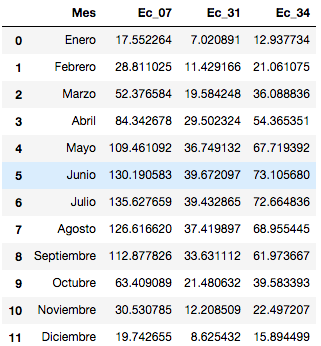
\includegraphics[width=0.65\textwidth]{figura5.png}
\end{figure}
\subsection{PARTE TRES}
En esta parte se utiliza el archivo de datos de flujos, básicamente en esta actividad se necesita generar una variable tipo datetime utilizando los días y horas que se presentan en el archivo. Para obtener columnas de horas y minutos a partir de los datros obtenidos se utiliza:
\begin{verbatim}
    
hora = []
minuto = []

for i in range(0,len(df2)):
    if (len(str(df2['Hour'][i]))==1):
        hora.append(str(df2['Hour'][i])[0:1])
        minuto.append('00')
        
    if (len(str(df2['Hour'][i]))==2):
        if (str(df2['Hour'][i])[0:2]=='24'):
            hora.append('00')
            minuto.append('00')
        else:
            hora.append(str(df2['Hour'][i])[0:2])
            minuto.append('00')
            
    elif (len(str(df2['Hour'][i]))==3):
        hora.append(str(df2['Hour'][i])[0:1])
        minuto.append('30')
    elif (len(str(df2['Hour'][i]))==4):
        hora.append(str(df2['Hour'][i])[0:2])
        minuto.append('30')
      
      
dia = []

for i in range(0,len(df2)):
    d = df2['DoY'][i]
    dia.append(d)
\end{verbatim}
De esta manera,  se puede generar un DataFrame de dias, horas y minutos y a continuación se necesita cambiar la manera de contar los dias tal que cambien cada vez que pasen 24 horas. Por último para crear la variable de Fecha se usa:
\begin{verbatim}
    Fecha = []
for i in range(0,len(df2)):
    date = '2018 '+str(dhm['DIA'][i])+ ' '+ dhm['HORA'][i]+ ' '+dhm['MINUTO'][i]
    Fecha.append(date)

FECHA = []
for i in range(0,len(df2)):
    d=datetime.datetime.strptime(Fecha[i],'%Y %j %H %M')
    F = d.isoformat(' ')
    FECHA.append(F)
    
df2['FECHA']=FECHA
df2.head()

df2['FECHA'] = pd.to_datetime(df2.apply(lambda x: x['FECHA'], 1), dayfirst=True)
df2 = df2.drop(['Year','DoY','Hour'], 1)
\end{verbatim}
Ahora se generan las columnas de mes, dia y horas y se agregan al DataFrame. Una vez haciendo eso, se modifican las variables tal que se encuentran los promedios de radiación neta, calor latente y calor sensible usando:
\begin{verbatim}
    df2["Rg_f_prom"] =df2.groupby(["MES","DIA","HORA"])["Rg_f"].transform("mean")
df2["LE_f_prom"] =df2.groupby(["MES","DIA","HORA"])["LE_f"].transform("mean")
df2["H_f_prom"] =df2.groupby(["MES","DIA","HORA"])["H_f"].transform("mean")

df2=df2.drop_duplicates(subset=["Rg_f_prom",'LE_f_prom','H_f_prom'])
\end{verbatim}
Después, se selecciona el mes de Diciembre y se muestra en la Figura 6 el balance de energía para tal mes utilizando:
\begin{verbatim}
    # BALANCE DE ENERGÍA PARA DICIEMBRE
Y1 = DIC['Rg_f_prom']          
Y2 = DIC['LE_f_prom']          
Y3 = DIC['H_f_prom']        

plt.plot(Y1, label = "Rg_f", color = 'darkorange')   
plt.plot(Y2, label = "LE_f", color = 'darkred')   
plt.plot(Y3, label = "H_f", color = 'seagreen')   
plt.xlabel("Horas")   
plt.ylabel("Energía")  
plt.legend()
plt.grid()
plt.title('BALANCE DE ENERGÍA PARA DICIEMBRE')
plt.show()
\end{verbatim}
\begin{figure}[ht]
\caption{Balance de energía para Diciembre}
\centering
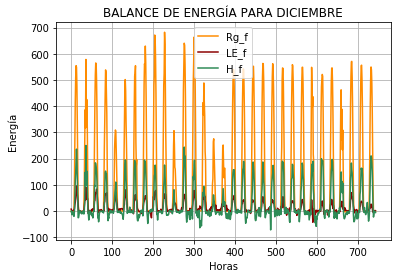
\includegraphics[width=0.65\textwidth]{figura6.png}
\end{figure}
Haciendo un DataFrame para el primer dia de diciembre, se observa el balance de energía para el primero de Diciembre en la Figura 7 utilizando:
\begin{verbatim}
    # BALANCE DE ENERGÍA PARA EL PRIMERO DE DIC.
h = []
for i in range(0,24):
    e=24
    h.append(e)

X = h                 
N = np.arange(24)         
Y1 = DIC1['Rg_f_prom']     
Y2 = DIC1['LE_f_prom']     
Y3 = DIC1['H_f_prom']      


plt.plot(Y1, label = 'Rg_f_prom', color = 'darkorange')   
plt.plot(Y2, label = 'LE_f_prom', color = 'darkred')   
plt.plot(Y3, label = 'H_f_prom', color = 'seagreen')   
plt.xlabel("Horas")   
plt.ylabel("Energía")  
plt.legend()
plt.grid()
plt.title('BALANCE DE ENERGÍA PARA EL PRIMERO DE DICIEMBRE')
plt.show()
\end{verbatim}
Por último se hace un nuevo DataFrame para el promedio de hora en Diciembre utilizando:
\begin{verbatim}
# nuevo dataframe para promedio de hora en Diciembre
DICPROM = pd.DataFrame()
DICPROM['HORA'] = DIC['HORA']
DICPROM['FECHA'] = DIC['FECHA']
DICPROM["Rg_f_prom"] =DIC.groupby(["HORA"])["Rg_f_prom"].transform("mean")
DICPROM["LE_f_prom"] =DIC.groupby(["HORA"])["LE_f_prom"].transform("mean")
DICPROM["H_f_prom"] =DIC.groupby(["HORA"])["H_f_prom"].transform("mean")
DICPROM=DICPROM.drop_duplicates(subset=["Rg_f_prom",'LE_f_prom','H_f_prom'])

\end{verbatim}
\begin{figure}[ht]
\caption{Balance de energía para el primerio de Diciembre}
\centering
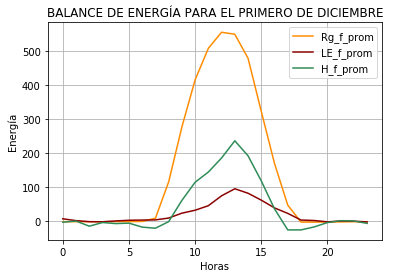
\includegraphics[width=0.65\textwidth]{figura7.png}
\end{figure}
Se muestra En la Figura 8 el balance de energía para el mes de Diciembre usando:
\begin{verbatim}
    # BALANCE DE ENERGÍA PARA EL MES DE DICIEMBRE
X = h                 
N = np.arange(24)         
Y1 = DICPROM['Rg_f_prom']     
Y2 = DICPROM['LE_f_prom']     
Y3 = DICPROM['H_f_prom']      


plt.plot(Y1, label = 'Rg_f_prom', color = 'darkorange')   
plt.plot(Y2, label = 'LE_f_prom', color = 'darkred')   
plt.plot(Y3, label = 'H_f_prom', color = 'seagreen')   
plt.xlabel("Horas")   
plt.ylabel("Energía")  
plt.legend()
plt.grid()
plt.title('BALANCE DE ENERGÍA PARA EL PRIMERO DE DICIEMBRE')
plt.show()
\end{verbatim}

\begin{figure}[ht]
\caption{Balance de energía en Diciembre}
\centering
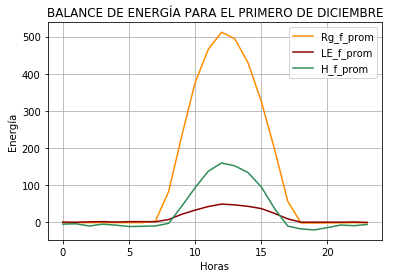
\includegraphics[width=0.65\textwidth]{figura8.png}
\end{figure}
\end{document}
